\subsection{题目描述}
\noindent The radial wave function of the 3s orbital is given by:

\[
R_{3s}(r) = \frac{1}{9\sqrt{3}} \times \left( 6 - 6 \rho + \rho^2 \right) \times Z^{3/2} \times e^{-\rho/2},
\]

where:
\begin{itemize}
    \item \( r \): radius expressed in atomic units (1 Bohr radius = 52.9 pm),
    \item \( e \approx 2.71828 \),
    \item \( Z \): effective nuclear charge for that atom,
    \item \( \rho = \frac{2 Z r}{n} \), where \( n \) is the principal quantum number (3 for the 3s orbital).
\end{itemize}

Compute the integral \( \int_0^{40} \left| R_{3s} \right|^2 r^2 \, dr \) for a Si atom (\( Z = 14 \)) using Simpson's rule with two different radial grids:

\begin{enumerate}
    \item[(1)] \textbf{Equal spacing grids}: 
    \[
    r[i] = (i - 1) h, \quad i = 1, \dots, N
    \]
    Try different values of \( N \).
    
    \item[(2)] \textbf{Non-uniform integration grid}: more finely spaced at small \( r \) than at large \( r \):
    \[
    r[i] = r_0(e^{t[i]} - 1), \quad t[i] = (i - 1) h, \quad i = 1, \dots, N
    \]
    Typically, choose \( r_0 = 0.0005 \) a.u. (1 a.u. = 1 Bohr radius).
\end{enumerate}

Discuss the efficiency of each approach and explain the reasons.

\subsection{程序描述}
待积函数为电子径向分布函数,理论结果应该十分接近全空间积分值$1.$使用Mathematica\textsuperscript{\textregistered}可以计算出不同积分终点$r_m$的定积分值
\[
    I(r_m) = 1 - \frac{1}{6561} e^{-\frac{28 r_m}{3}} \left( 6561 + 28 r_m \left( 2187 + 14 r_m \left( 729 + 392 r_m^2 \left( 81 + 28 r_m \left( -9 + 14 r_m \right) \right) \right) \right) \right)
\]
对于本题终点$r_m = 40$的积分值为
\[
I(40) = 1 - \frac{1}{6561} e^{-\frac{1120}{3}} \cdot 242794431087524801 \approx 1 - 2.7 \times 10^{-149}
\]
积分步骤与结果详见\texttt{src/theoretical.nb}。 
原始的Simpson积分法源自等距节点的Newton–Cotes公式,因此在第$2$问使用非均匀节点计算时,需要给积分核\(\left| R_{3s} \right|^2 r^2\)乘上换元因子\(dr = r_0 \cdot e^{t}\),本质是转换成了新的定积分$g(t)$在等距节点$t$上的Simpson积分。

源代码在\texttt{src/simpson.py}中,其中的\texttt{integrand}函数即为原始积分核,\texttt{simpson\_rule}为基于给定点与函数值的Simpson积分法的实现。主程序中,在$N=[3, 5, 7, 9, 11, 21, 51, 101, 201, 501, 1001, 10001]$分别计算了两种节点下的积分值。实际上在实现\texttt{simpson\_rule}的时候,对传入的偶数节点数进行了舍尾处理,增强了程序的健壮性。在\texttt{src}中,运行\ccmd{python -u simpson.py}即可得到结果,需要安装\texttt{numpy}与\texttt{matplotlib}库。
在随后的结果示例中,我们将看到,非均匀节点的积分值更快收敛于理论值。其根源在于坐标变换之后,采集点更密集地分布在积分核的峰值区域,避免了在积分核值较小的区域上的采样浪费。为了直观展现这一点,主程序选取了$N = [11, 51, 201, 1001]$进行点分布绘制,详见结果示例。
\subsection{伪代码}
\begin{algorithm}[H]
    \caption{Simpson's Rule Integration}
    \KwIn{$r(\text{array, shape}=N)$ $f(\text{array, shape}=N)$}
    \KwOut{$\text{integral}(\text{float})$}
    
    $N \gets \text{len}(r)$ \tcp*[r]{Number of grid points}
    \If{$N < 3$}{
        \KwRet \texttt{Error: Simpson's rule requires at least 3 points}
    }
    \If{$N \% 2 == 0$}{
        $r \gets r[:-1]$; $f \gets f[:-1]$; $N \gets N - 1$ \tcp*[r]{Ensure an odd number of points }
    }
    
    $h \gets \frac{r[N-1] - r[0]}{N - 1}$\;
    $S \gets f[0] + f[-1]$ \tcp*[r]{Notice index from 0 in python}
    
    $S \gets S + 4 \times \sum f[1 : -1 : 2]$ \tcp*[r]{Notice range in python excludes the last element}
    $S \gets S + 2 \times \sum f[2 : -2 : 2]$ \tcp*[r]{Add 2 times sum of even-indexed terms}
    
    $\text{integral} \gets \frac{h}{3} \times S$

    \KwRet $\text{integral}$
    \end{algorithm}
    
\subsection{结果示例}
\begin{figure}[H]
    \centering
    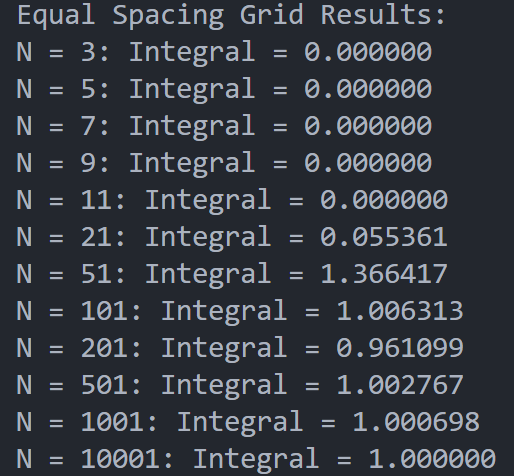
\includegraphics[width=0.45\textwidth]{Problem_3/figs/terminal_1.png}
    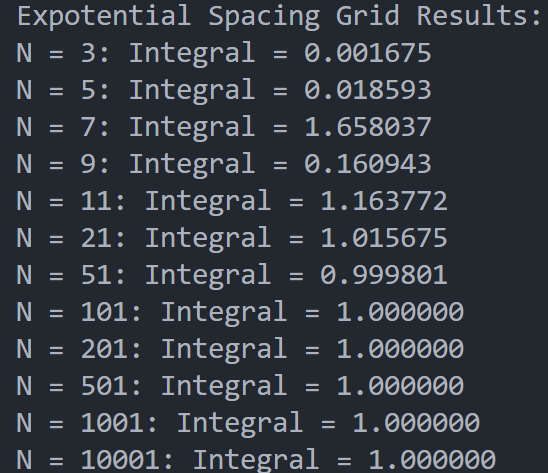
\includegraphics[width=0.48\textwidth]{Problem_3/figs/terminal_2.png}
    \caption{两种节点比较}
\end{figure}

\begin{figure}[H]
    \centering
    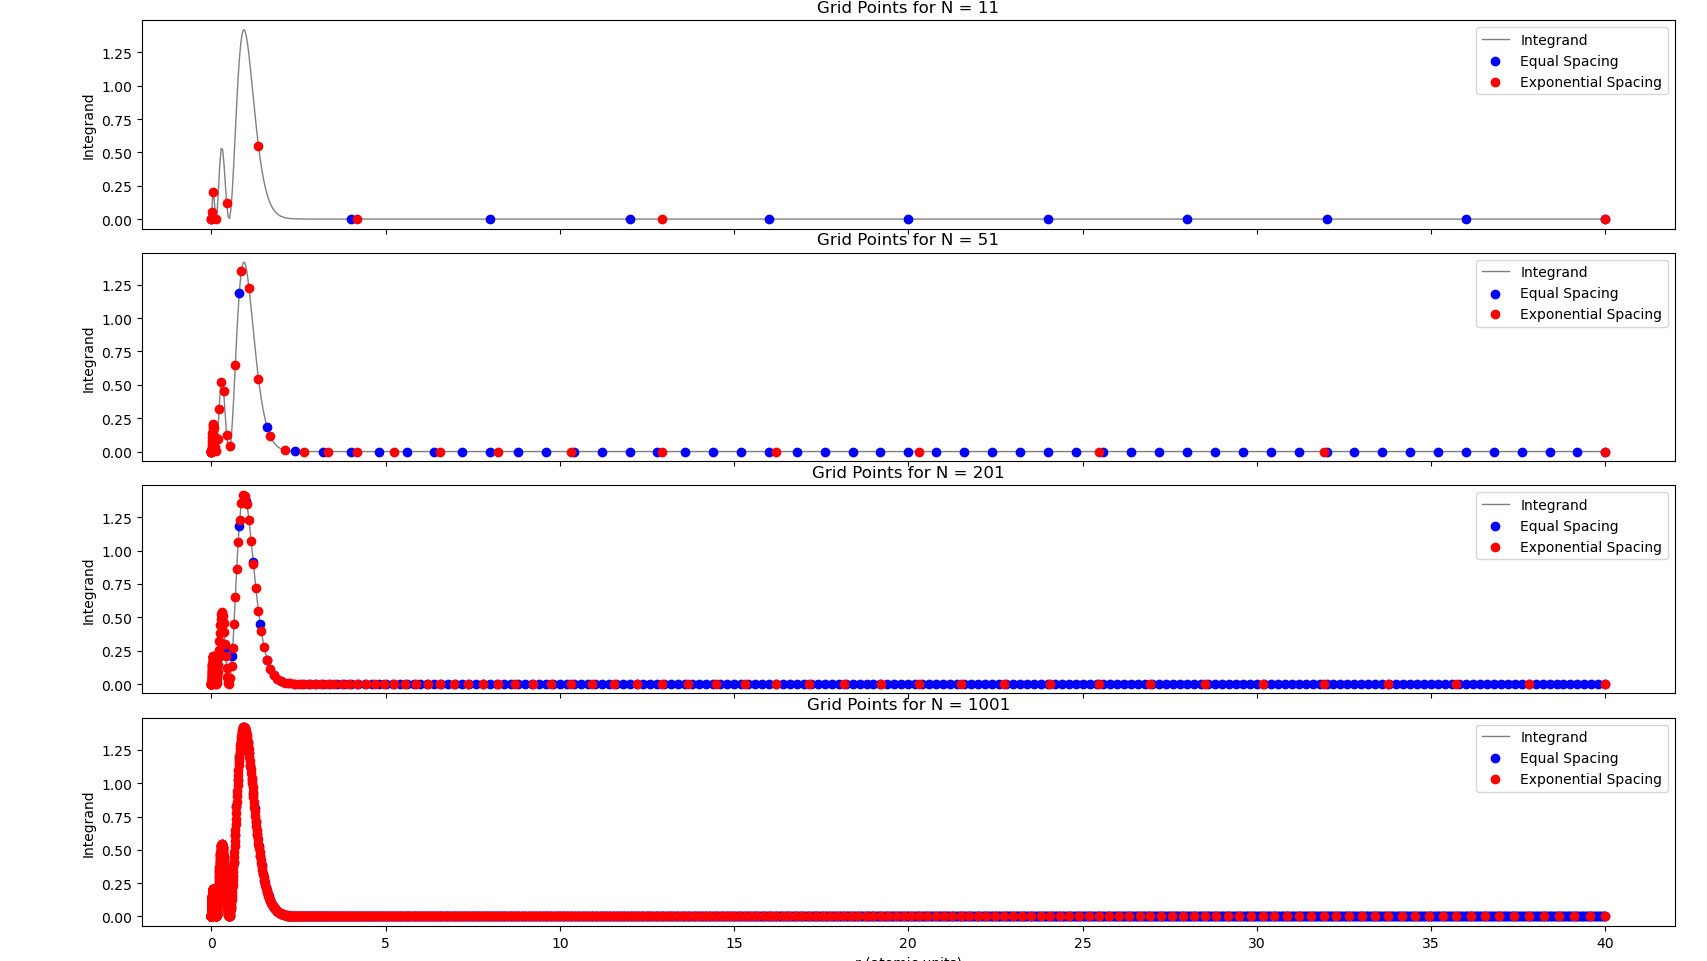
\includegraphics[width=1.0\textwidth]{Problem_3/figs/nodes.png}
    \caption{不同节点取样分布对比}
\end{figure}

